\clearpage
\lhead{\emph{Chapter 5: TRACS upgrade, description and implementation}}  % Set the left side page header to "Symbols"
\chapter{TRACS upgrade, description and implementation}
% I'm missing the general approximations made in TRACS such as no electron-electron interaction
\label{chap:tracs}

%We have already stated the importance of simulating software in research in general and in radiation damage studies in particular, so it should come as no surprise that this next chapter is entirely dedicated to the software developed during this project. 
According to speed and accuracy of simulation software, we could classify it in 2 categories: fast light-weight approximate simulators or slow, powerful, accurate simulators. The latter group being used for device design and performance prediction and the fast simulators commonly used for measurement comparison in laboratory situations.

Here we will focus on the fast and light-weight simulators since that is the software that was upgraded during this project. 

% Confirm with Marcos before writting why we don't use others
In the silicon detector simulation field, specially amongst members of the RD-50 collaboration from CERN \cite{RD50}, there were several already available simulators capable of reproducing TCT measurements for different detector configurations (diode, micro-strips\ldots) each of them (kDetSim, Weightfield2...) with some additional features. The software of choice for this project was the Transient Current Simulator (TRACS) developed by Pablo De Castro\footnote{Former Student of Universidad de Cantabria} in 2014 in the PH-DT-DD-SSD group at CERN. 

The reason to use TRACS was based on two arguments. First one is that TRACS is an open-software platform built around efficient open-software libraries that have been exhaustively tested and validated by third parties. And second and probably more important is that the software TRACS was already developed and used in the PH-DT-DD-SSD group with future improvement in mind such as the one realised in this project.

In this chapter we will present the structural design of the software as it was before the project started including the different parts in which it is divided. This chapter is also intended to serve as additional documentation of TRACS. We will also present the changes and upgrades performed with particular emphasis on the implementation of radiation damage. Finally, we shall comment briefly on where the software stands now, after the upgrades, and what further improvements could be made.

\section{Software design} % (fold)
\label{sec:softDesign}

TRACS is built and written in C++11 ISO standard \cite{C++11} and makes use of Fenics \cite{Fenics} and Boost libraries \cite{Boost} for calculations and Qt \cite{Qt} and VTK \cite{VTK} for GUI, plotting and visualisation. The whole software takes advantage of Object Oriented Programming and it is, thus, organised in different classes. TRACS also has two different operational modes available: a command line interface (CLI) and a Graphical User Interface (GUI) both of which will be explained in detail later in this section.

During a typical simulation of TRACS, the program takes detector properties (thickness, depletion voltage, geometry...) and carrier position (the laser is modelled by the charge deposition it produces). TRACS then solves Poisson's equation for the given conditions to obtain the electric field. This part is done using the aforementioned Fenics libraries taking advantage of their efficient PDE solver. Then the carriers are allowed to drift inside the detector using the electric field obtained in the previous step; Ramo's theorem is used to calculate the induced signal in the circuit. Waveforms are saved and stored in both plain text and ROOT\cite{ROOT} format. This process is shown in Figure \ref{fig:TRACS_fc} as a flow chart; some of the components of TRACS will be explained in detail in the following section.

\begin{figure}[H]
	\centering
	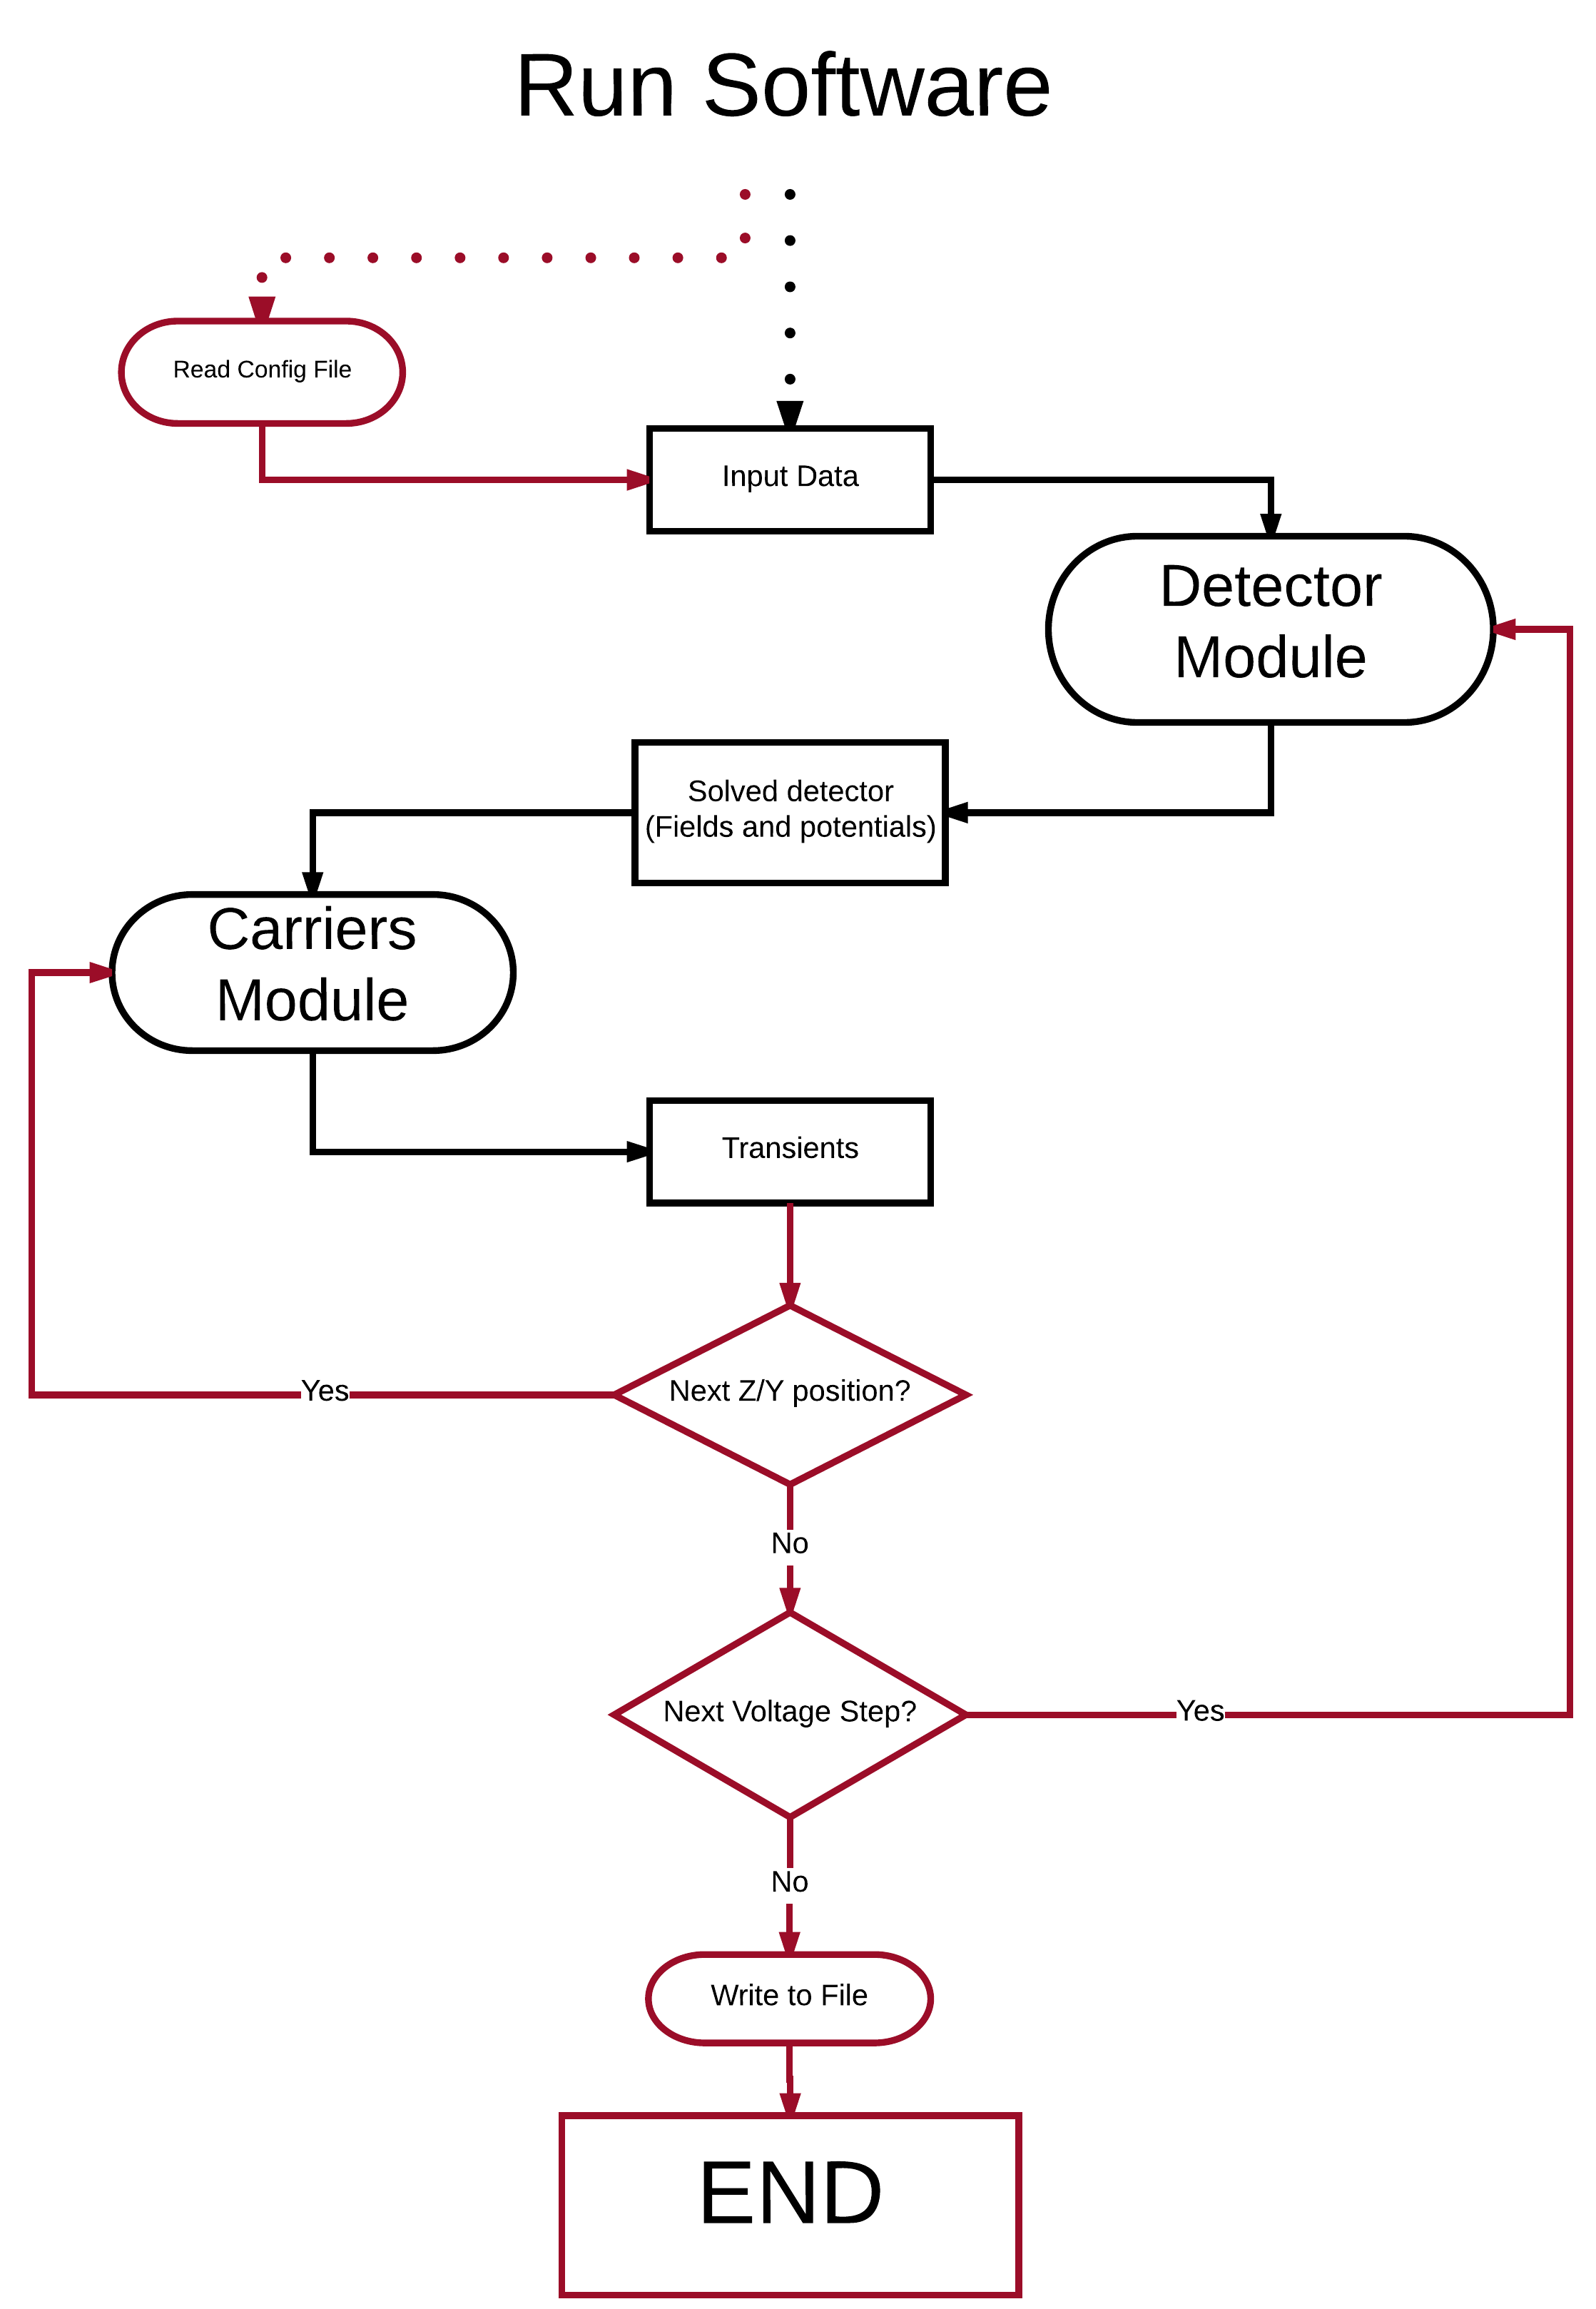
\includegraphics[width=0.9\textwidth]{TRACS_fc.png}
	\caption{Flow chart of the most general voltage and coordinate scan implemented in TRACS. It includes Command Line Interface only parts (dark red) and parts present in CLI and graphical mode as well. It is a simplified view of the simulation process. Rounded shapes represent processes and rectangles represent the intermediate results.}
	\label{fig:TRACS_fc}
\end{figure}

Talk with MARCOS %This behaviour was present in the original version of TRACS an still remains at the core of every simulation performed using the software. Now we will briefly summarise the different parts that compose TRACS from its original state to the latest upgrade.

\subsection{Detector module and Partial Differential Equations solver}

\begin{figure}[H]
	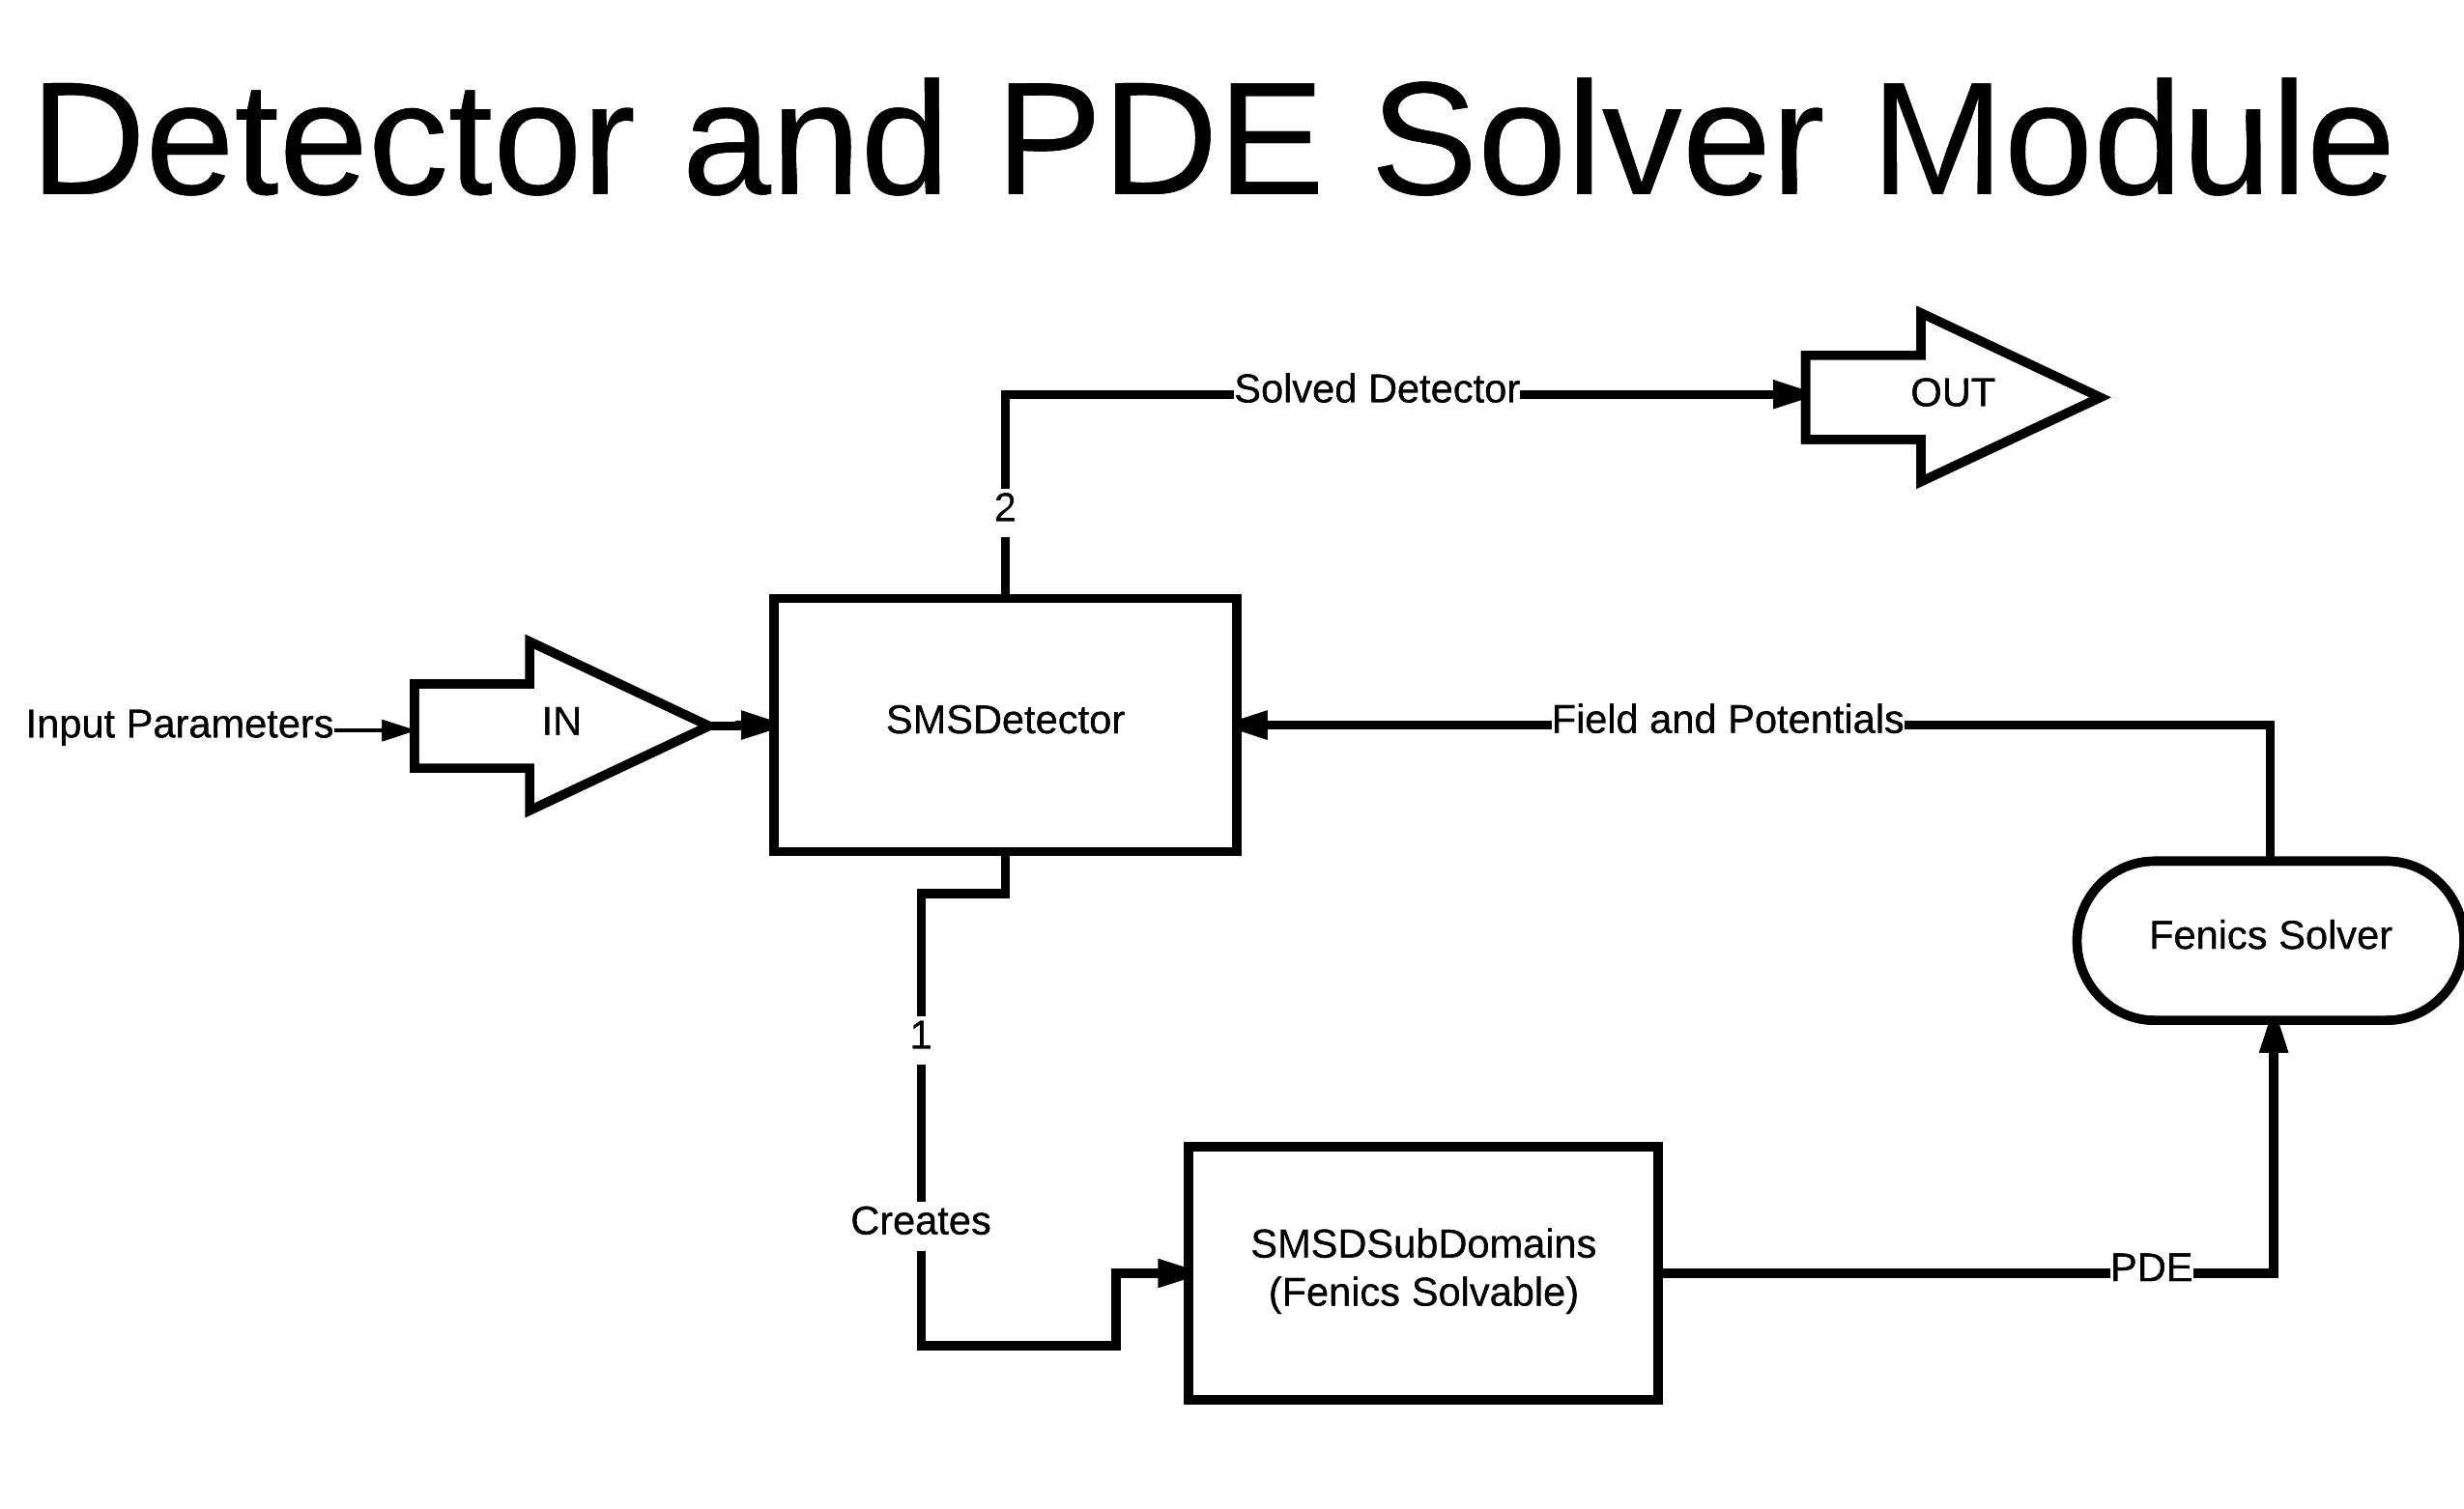
\includegraphics[width=0.9\textwidth]{Detector_Module.png}
	\caption{Flow chart of the behaviour of the so-called Detector Module. This is a simplified representation of the process by which the detector is initialised and the fields and potentials inside are calculated.}
	\label{fig:DetectorFc}
\end{figure}

One of the core modules of TRACS is that composed of the detector class and PDE solver which has been called "Detector Module"; its behaviour is depicted in Figure \ref{fig:DetectorFc}. The main classes of the module are \textit{SMSDetector} and \textit{SMSDSubDomains}. In the first, detector properties (geometry, electric field inside...) are stored as attributes that allow the class to represent a detector. The class \textit{SMSSubDomains} serves as a bridge between the \textit{SMSDetector} class and Fenics solver; geometry and boundary conditions are stored inside of it in such a way that Fenics solver is capable of understanding and solving the PDE. 

The PDE solving algorithm is fully provided by Fenics libraries and the configuration done through \textit{Poisson.h} and \textit{Gradient.h} files. The electric and weighting potentials and fields obtained after solving Poissonś equation are stored in the class \textit{SMSDetector} as attributes of Fenic's internal type \textit{Function} and are accessible through public \textit{getter} methods.

If several simulations are to be performed using the same detector and initial conditions, the fields and potentials need not be calculated since they are saved in memory by TRACS. 

This part of the software is flexible enough to accommodate for any detector geometry with few changes in the code, thanks to the use of Fenics. Diodes and micro-strips are simulated out-of-the-box. In particular, diodes are considered a special case of micro-strips with just one strip covering the entire surface of the detector.

It is in this part of the software that \neff is calculated through the value of $V_{dep}$ for the non-irradiated case, see equation \ref{eq:widthVias}. Several modifications were done in TRACS to extend its capabilities of simulation to a radiation-modified \neff parametrisation decided by the user. We will explain the modifications in the next section as we go through the modifications performed to TRACS.


\subsection{Carriers Module and drifting}

\begin{figure}[H]
	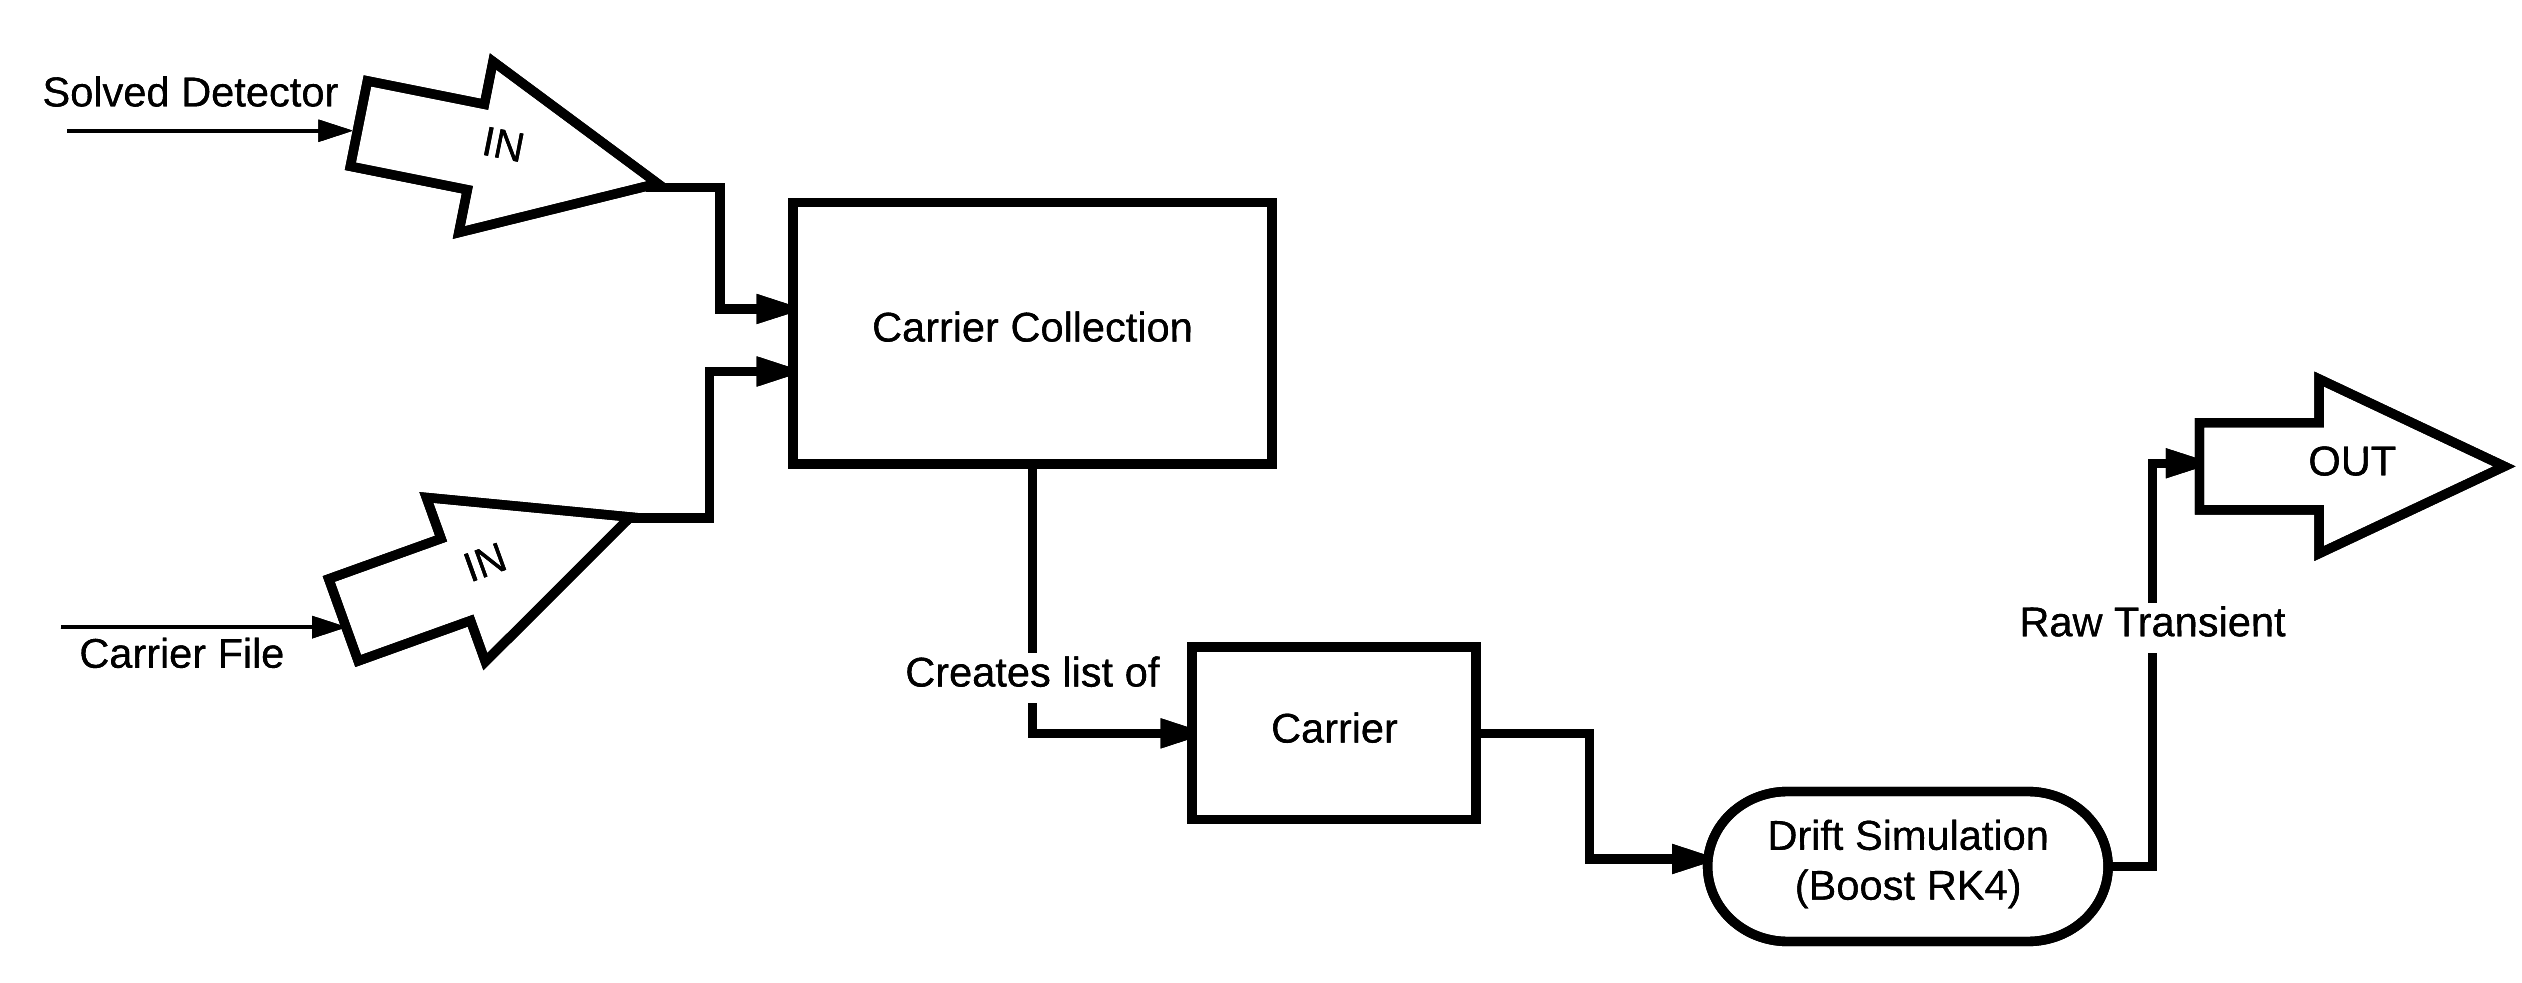
\includegraphics[width=0.9\textwidth]{Carriers_Module.png}
	\caption{Flow chart of the behaviour of the Carriers Module is presented. This is a simplified view and doesn't show all the classes present in the module as it is intended only to represent the behaviour of the module.}
	\label{fig:CarrierFc}
\end{figure}

After the electric and weighting fields and potentials have been calculated, the software proceeds to move the charge carriers inside the detector. This is handled by the classes: \textit{CarrierCollection}, \textit{Carrier}, \textit{CarrierMobility}, \textit{CarrierTransport}. A flow chart of the behaviour of this module can be seen in Figure \ref{fig:CarrierFc}.

The charge carriers are input via an ASCII file automatically produced for the user using python scripts. The scripts are not distributed with TRACS but carriers files can be created by users following the current format. The carriers file contains one carrier per line with initial position (in the 2-D section of the detector), the off-set time at which they should be generated in the simulation, and the equivalent charge they carry. The carriers can be moved about the detector if needed so that the user does not need to simulate the movement of the laser. The current is calculated using Ramo's theorem for every carrier and added together for every time step.

A time offset in the input file is used to shift the start position of the waveform. This is useful to match the measured and simulated waveforms.

%The off-set generation time introduced as an input is a quantity whose actual value is of no significance and it is only introduced to reproduce better the waveforms obtained in the lab, specially the first spike that appears as the carriers are created and the signal in the circuit starts to be collected. 

% maybe use equations here?
An important feature of the TRACS carriers simulation is the grouping and splitting of carriers by assignment of a weighted charge. This means that groups of charge carriers  of the same type, lying initially very close together, can be simulated as being just one charge carrier with a total charge equal to the sum of all the individual charges of the carriers. This reduces greatly the number of individual charge carriers that need to be simulated hence improving simulation times. This grouping can be done with almost no penalty in precision of the results as carrier-carrier interactions are neglected.

Simulating the movement of carriers inside the detector requires to solve the first order differential equation\cite{PdeCastro}\[\frac{d\vec{x}(t)}{dt} = \vec{v}(t) = \mu \vec{E}(\vec{x}(t))\]That is taken care by Runge-Kutta-4 method implemented inside ODEINT libraries. ODEINT libraries now come as a standard part of BOOST libraries inside C++11. These libraries, together with Fenics, ensure fast, efficient and robust computational properties at the core algorithms.



\subsection{Joining all together (CLI and GUI)}

To bring all the components together TRACS has both a CLI and a GUI available to the user. TRACS is designed around two main use case scenarios: quick checks and long simulations. For the latter case CLI was designed, providing the user with an easy, low resource execution version, that can be easily automated. 

\subsection{GUI and its advantages}

\begin{figure}[H]
	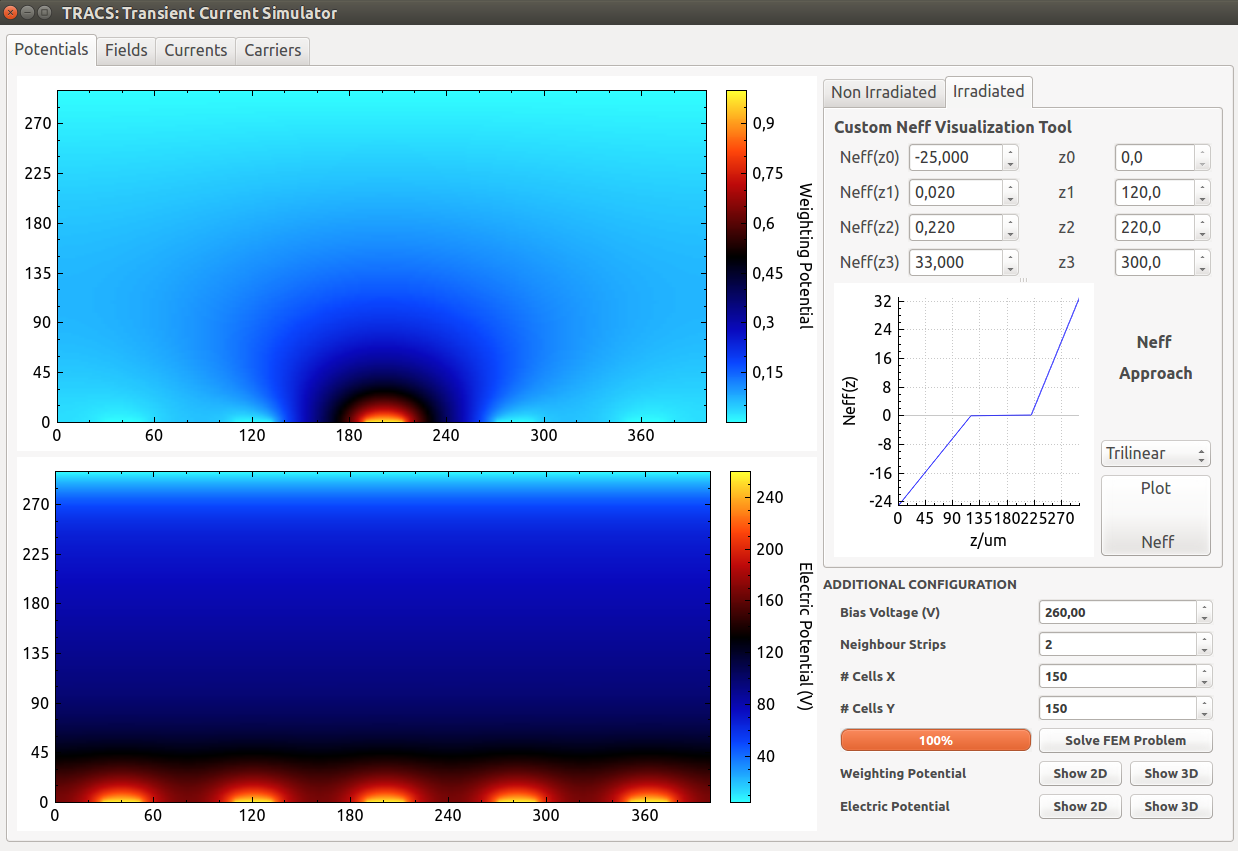
\includegraphics[width=0.9\textwidth]{TRACS_CNVT.png}
%\begin{flushleft}
	\caption{Screen-capture of TRACS' GUI. The GUI provides 4 different tabs that allow for easy and fast simulation of various scenarios including single particle, line of carriers and custom carrier distribution. The tab shown here shows the interface for parameter input and detector solving.}
%\end{flushleft}
	\label{fig:TRACSGUI}
\end{figure}

Besides the already mentioned CLI, TRACS also provides a GUI (see Figure \ref{fig:TRACSGUI}) to allow for easy checks and a more user-friendly approach to simulations. It is divided in different tabs for each of the different components of TRACS.

First tab allows the user to configure all the detector parameters and solve the PDEs for the specific detector parameters. After resolution of the PDEs, all the potentials and fields are plotted inside the potentials tab and the fields tab respectively. The graphs offer colour-coded 2D maps as well as 1D cut of the fields; interactive 3D plots are also available through VTK tools.

The other two tabs are used for carrier drifting and waveform simulation. Options range from 1 carrier simulations and simulation of a line of carriers to full laser illumination simulations (provided that an externally generated file is present). The Carrier tab is equipped with a carrier visualisation window (to display the carrier generation shape) and a waveform visualisation window (to study the simulated induced current). TRACS-GUI also allows saving the waveforms in plain text format.

\subsection{Approximations and limits of TRACS} % Necesito ayuda para maquillar el titulo
\label{sec:approxTRACS}

TRACS needs to make some approximations to reduce the computational requirements of the simulations. A rough 10\% precision loss can be estimated from these approximations, when compared to real data. % This approximations could, in principle, compromise the precision of TRACS results but it has been seen that in normal use case scenarios TRACS is capable of matching accurately the data\cite{TRACSCompar}.
 
TRACS solves internally the necessary PDEs in 2D only because a planar detector can be approximated as being a 2D structure. However, because TRACS makes use of Fenics libraries it is possible to implement 3D detectors in the future if required.

Another approximation made by TRACS is neglecting any electron-electron (or hole-hole) interactions inside the detector. It is a justified since the $\overrightarrow E$ inside the detector are many orders of magnitude greater than the $\overrightarrow E$ due to all the carriers.

The thermal diffusion of charge carriers inside the detector is also neglected in TRACS. The thermal diffusion is mostly important in the undepleted bulk. In the depleted zone it adds a smearing of few microns to the final position of the carriers. A consequence of this simplification is that TRACS is only accurate when simulating fully depleted detectors. 

\section{TRACS upgrade} % (fold)
\label{sec:devTRACS}

All the modules and features we have explained in the previous section were part of the original TRACS software. From that point the software was modified and upgraded to \emph{1)} include radiation damage effects  with user defined parameters and \emph{2)} improve the usage of TRACS both as a standalone and as a library-like module for bigger projects.

%All the changes made during this project were oriented to either the main goal: Implementing radiation damage into the simulations; or future extensibility of TRACS capabilities. These future oriented features will be commented briefly since they are not a fundamental part of the project and most of the information regarding them will lay under future projection or future upgrades proposal.

%The radiation damage effects that were implemented and represent the core of the project will be explained in detail with detailed explanations on the specific decisions that were made and how the implementation was done. This will be separated in two parts dividing the physics part and rationale from the coding and software design part of the whole implementation.

\subsection{Modifications to TRACS}

The different effects of radiation damage in the signal obtained from a silicon detector have been discussed before and we concluded that besides the change in $V_{dep}$ and leakage current, the main effects were the loss in charge collection efficiency and the modification in the shape of the waveform due to the perturbated \neff. These effects are all the result of the Vacancy-Interstitial defects in the lattice due to particle-Si collisions.

%For TRACS simulation capabilities, the increase in leakage current needs not be taken into account. This leaves only increase in $V_{dep}$, \neff modification and trapping of carrier to be implemented inside the code. The increase in $V_{dep}$ can be included in the \neff modification since $V_{dep}$ is dependant on the \neff inside the detector so that by solving the PDEs for the modified \neff one should automatically obtain the correct $V_{dep}$ value.

%The \neff modification is, as we have already discussed, a rather complicated effect to implement in a simulator software like TRACS that cannot reproduce the irradiation process. It is then required to have a model for how the \neff get distorted from the original constant value as a function of radiation fluence. There is not such a model that works satisfactory for wide range of fluences, which leaves room for custom solutions. 

%It is important to know that one of the ultimate goals of the bigger TRACS project is to be used as part of a fitting tool that would take waveforms of irradiated silicon detectors as input and return the \neff configuration that yields the closest results. This way TRACS would greatly diverge from current silicon detector simulators in such a way that it can get information about the detector retrospectively on top of performing approximate simulation-prediction of what the results should be.

%This simplifies greatly the implementation process as it is not needed to use any approximate model that would parametrise trapping and \neff modification effects as a function of the radiation fluence the silicon detector has be subject to. This models often require multiple experimental coefficients that may vary under different conditions and one might end up needing to use several different models to fully parametrise just one physical value. The approach taken in this project sits on the opposing end, rendering TRACS viable to be used as another analysis tool as well as a guessing/comparing tool.

In TRACS three models for the change of \neff with fluence were included.The first one, the linear approximation, has only 2 free parameters that would need adjusting. This parametrisation has given good results in modelling \neff modification in irradiated silicon detectors.

The second modelling of the \neff (already introduced in section \ref{sec:trapEfect}) consists on 3 different areas where the carrier density is constant. 
The third model is a combination of the two previous models. The \neff configuration is assumed to have three different zones in which it is linear with depth. %This two last approximations require that restrictions are imposed in the allowed values for each zone so that continuity and derivability are ensured.

In the linear approximation, continuity and derivability are guaranteed as it consists of only one straight line. Derivability, though not strictly necessary for current use of TRACS, has been ensured in both triple linear and triple constant approximations by means of hyperbolic tangents connecting the end of one area with the beginning of the adjacent one. Continuity in the triple constant approximation arises from these hyperbolic tangent bridges that connect smoothly one value of the \neff in one area to the vale in the next; in the triplelinear case continuity is forced because the parametrisation requires that adjacent \neff zones have the same value at the interface point. 

Trapping of charge carriers is a statistical process and it would require for each carrier, a probability evaluation after each step with the corresponding performance penalty, specially for low trapping probabilities and high number of carriers.

To avoid such computational overhead, we opted for the approximated implementation of the effect through the use of an exponential wrapping over the whole waveform. The physical justification of the approximation has already been explained in section \ref{sec:signalDeg}. This approximation requires enough simulated time and enough carriers to be accurate enough.

The last of the upgrades to TRACS was the inclusion of electronics shaping. TRACS had lowpass filter shaping as an option in CLI version but that was not good enough for detailed comparisons to measured data. We implemented electronics shapping by convoluting the raw signal (or the low pass filtered one) with the amplifier transfer function. %The transfer function is specific to the amplifier.

% On top of the improvements we have mentioned, that were oriented mainly to include radiation damage into the simulations, some other features have been implemented with focus on user experience or future development of TRACS. These features are of less importances for the research project but equally important for TRACS and its future projection. 

% A common charasteristic of these \textit{side features}, as we may call them, is that none of them increase performance, accuracy\ldots of TRACS but make it easier to be used, modified, understood\ldots Amongst these features we can find improvements such as better comments and code clean-up and the improvements on the README text file that includes now a more detailed installation guide as well as a quick-guide for the most typical use case scenarios.  Also 

Another important change to the CLI was the addition of a configuration file was added to the code, together with the necessary \textit{parser}, eliminating the need for recompilation every time an input value is changed, and making it possible for users to change simulation parameters in CLI without the need to dig into the code. The code (existing and new) was also commented and documented.

TRACS execution options were expanded with the inclusion of the new class \emph{TRACSInterface} that allows the simulation to be called as a a library from an external user code.

%The last addition to TRACS is the ability to be used and integrated into bigger software (e.g.: ROOT) as a library package. This was achieved by the development of \textit{TRACSInterface}, a class that acts as the bridge between any software and TRACS.

The \textit{TRACSInterface} class contains a simple set of methods that allows the user to read the input values from the configuration file, modify those parameters and perform every step of the whole simulation as well as returning results. The creation of this library avoids compilation of TRACS sources every time the user code is to changed.

\subsection{Implementation of TRACS upgrade}

Implementation of the improvements in TRACS did not present any significant design problems due to the usage of Object Oriented programming and external flexible libraries. In the case of modified \neff implementation Fenics libraries provide users with the option to define a custom space charge distribution to solve Poisson's equation. 

By creating a new class \textit{Source} the \neff could be parametrised. Inside the class, \emph{Setter} methods were also implemented so that \neff approximation and parametrisation can be modified at run-time. By having a dedicated class for \neff parametrisation TRACS can also be easily extended to account for any other new parametrisations. 

%As we showed in equation \ref{eq:trapCurr} the trapping effects on the signal can be seen as an exponential wrapping of the non-trapped signal. For the implementation of the exponential wrapping of the waveform it suffices to multiply the raw values in each time step by the exponential factor at the given time. This simulates the effect of the statistical trapping and yields an exponential decrease in the output current that mimics the experimental one.

For both \neff parametrisation and trapping effects, it is needed for the user to input the relevant parameters. For the custom \neff effect the input data are the coordinates of the points needed to define the selected \neff parametrisation. The number of parameters needed in each case varies from 2 for the linear case to 5 for the triple constant \neff to 6 for the case of triple linear approximation. In the case of trapping effects, only one parameter is needed: $ \tau $.

The configuration file, \textit{Config.TRACS}, was added with its own syntax that allows the parser to distinguish input values from comments. % The \textit{TRACSInterface} development was done, as previously stated, on a new separate class in addition to the already present CLI and GUI so that nothing had to be change for standalone use of TRACS.

The GUI version of TRACS has also been upgraded to account and make use of the changes for simulating irradiated detectors. These changes include the extra fields to input the new parameters such as \neff parametrisation type and coordinates, trapping time and a toggle to switch between simulation of irradiated detectors or non-irradiated detectors. 

%It is an unintended feature of TRACS that one can de-couple \neff modification and trapping effects allowing the user to explore both effects separately by simply toggling on radiation simulation and inputing a constant \neff or a very big trapping time (i.e.: effectively no trapping). 
Other improvements to TRACS-GUI include the implementation of RC shapping capabilites for output waveforms as well as resizable plots throughout all tabs. The last of the visual improvements to TRACS is the inclussion of the Custom N$_{eff}$ Visualization Tool which allows the user to preview the \neff profile before starting the simulation.

\section{Summary}

TRACS has been improved and upgraded to include radiation effects into the simulations with user defined \neff and trapping parameters. On top of those improvements TRACS, documentation was also extended. Flexibility was added so that now TRACS can run as an additional library in an external user code.

The original version of TRACS showed excellent agreement with experimental data from laboratory measurements so it is expected that the new version of TRACS be a useful and accurate tool. This accuracy will be tested in the next section.%, that will prove TRACS usefulness as a research tool for anyone interested in radiation damage in silicon detectors.

